\documentclass[a4paper,11pt,openright,oneside]{report}
\usepackage[utf8]{inputenc}
\usepackage[T1]{fontenc}
\usepackage[portuguese]{babel}
\usepackage{graphicx}
\usepackage[backend=biber, style=ieee]{biblatex}
\usepackage{csquotes}
\usepackage{blindtext}
\usepackage[printonlyused]{acronym}
\usepackage{hyperref}
\usepackage{minted}
\usepackage[titletoc,title]{appendix}
\usepackage{caption}
\usepackage{subcaption}
\newcommand{\RNum}[1]{\uppercase\expandafter{\romannumeral #1\relax}}

\begin{document}

\title{\textbf{Comando Infra-Vermelhos no Controlo de LEDs}\\[1cm]\textsc{\small {Departamento de Electrónica, Telecomunicações e Informática} \\ \large {UNIVERSIDADE DE AVEIRO}}}
\author{Sandra Moreira 76471, Ricardo Jesus 76613\\simoreira@ua.pt, ricardojesus@ua.pt}
\date{6 de Maio de 2015}
\maketitle
\pagenumbering{arabic}

\chapter{Infra-Vermelhos no Controlo de LEDs}

\section{Especificação do Sistema}
\label{sec:especificação}

Irá ser utilizado o comando infra-vermelhos disponibilizado juntamente com o kit Terasic DE2-115 (ver \url{http://goo.gl/JYc7PE}, p. 98) de forma a controlar os seus LEDs verdes. Os dígitos do comando deverão controlar a quantidade de LEDs acesos enquanto que duas setas deverão controlar a sua intensidade luminosa. O botão de \verb|POWER| deverá colocar a máquina num estado inactivo, com todos os LEDs apagados, e retomar o seu estado quando premida novamente. Na secção \ref{sec:Manual} é possível consultar uma imagem (\ref{fig:ir_leds0}) explicativa do funcionamento do comando. 

O sistema deverá funcionar de acordo como o exemplificado na Figura \ref{fig:ir_leds1}

\begin{figure}[ht]
\center
\fbox{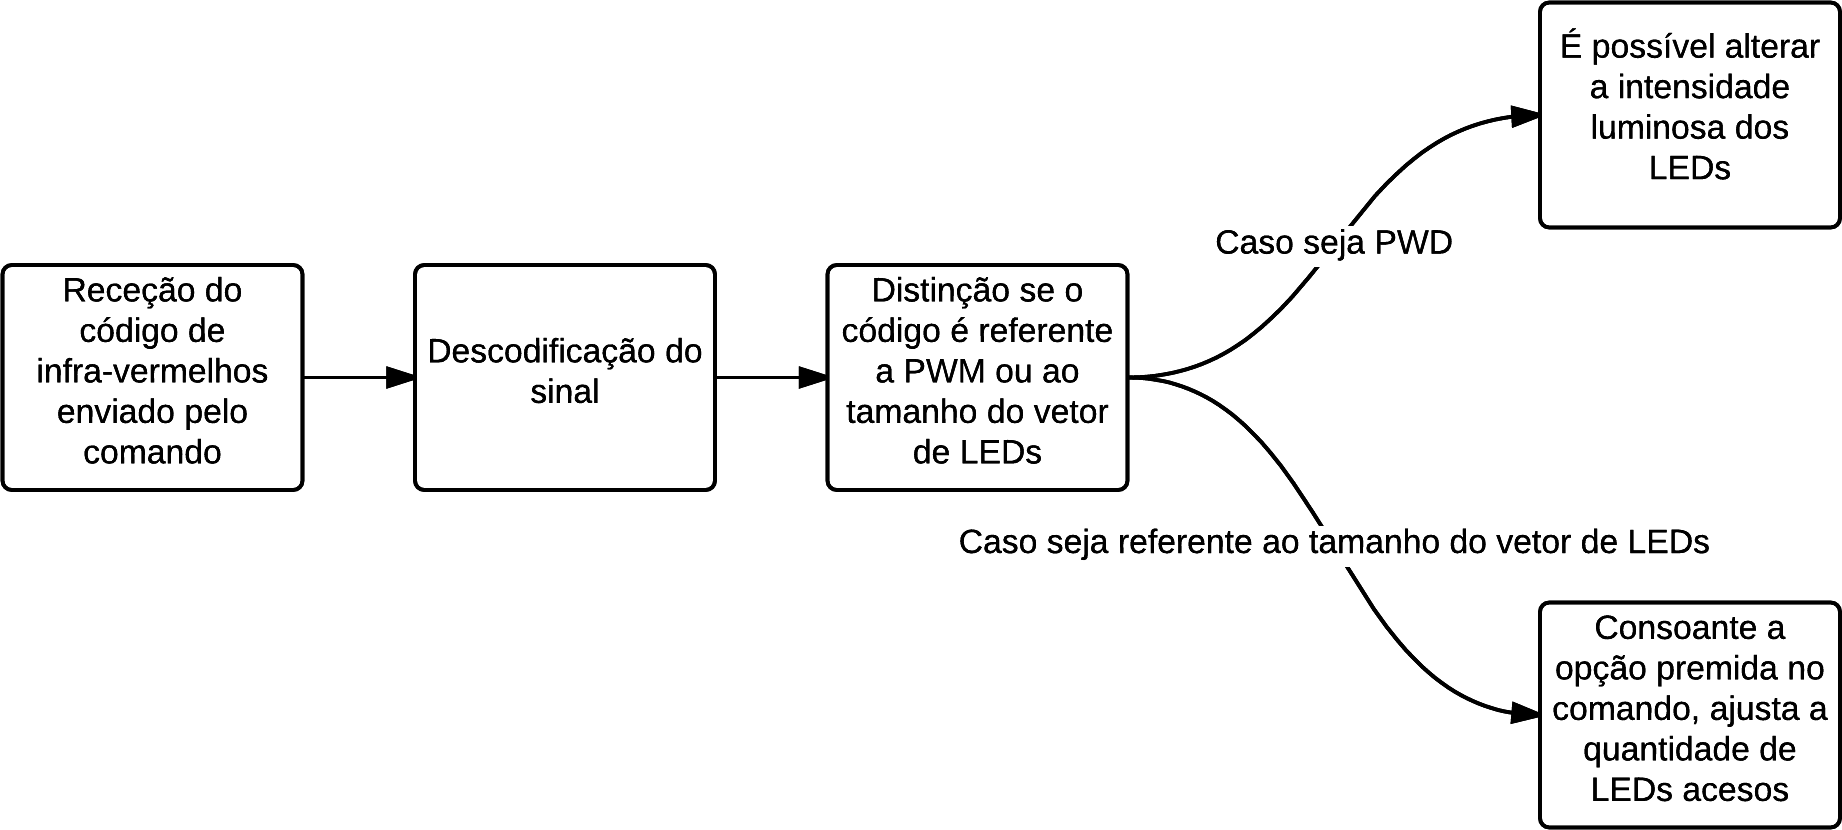
\includegraphics[height=5cm]{img/ir_leds1}}
\caption{Funcionamento do projecto desenvolvido}
\label{fig:ir_leds1}
\end{figure}

\section{Arquitectura do Sistema}


O sistema deverá funcionar conforme o especificado na Secção \ref{sec:especificação}, e indicado na Figura \ref{fig:ir_leds1}.

Desta forma pensou-se em recorrer aos blocos abaixo de forma a atingir este funcionamento. Atendendo a que a máquina terá essencialmente dois processos a correr em simultâneo (a definir a quantidade de LEDs acesos e a intensidade luminosa destes), optou-se por se dividir estas funções por dois ramos bastantes ``concretos'', cada um resolvendo uma parte do problema. O resultado final deverá ser a junção  dos resultados obtidos nestes caminhos. Um diagrama de blocos do projecto a desenvolver é ilustrado na Figura \ref{fig:ir_leds2}.

\begin{description}
\item[Recetor IR] Responsável por receber o código infra-vermelhos enviado pelo comando e transmitir para o resto da máquino um código de 8 bits, referente à tecla premida.
\item[Descodificador de IR] Responsável por receber um código de 8 bits e transmitir a cada um dos ramos correspondentes um código indicativo do que deverá ser levado a cabo. Um código pode dizer respeito à intensidade luminosa dos LEDs ou à quantidade de LEDs acesos.
\item[Contador PWM] Responsável por manter registo do valor de luminosidade em uso, e ajustá-lo conforme indicado: adicionando ou subtraindo uma unidade ao valor atual, guardando este valor e colocando a luminosidade a zero (ou vice-versa), ou simplesmente mantendo este valor sem alterações. É um bloco directamente controlado pelo \verb|Descodificador de IR|.
\item[Controlo PWM] Responsável por, recebendo um valor binário de 5 bits, controlar a intensidade luminosa dos LEDs através de \textbf{Pulse Width Modulation (PWM)}, técnica desenvolvida abaixo.
\item[Descodificador 5 bits - 7 Seg] Responsável por, recebendo um valor binário de 5 bits, transmitir dois vectores cada um de 7 bits com o valor correspondente em decimal construídos de forma a serem directamente utilizáveis em displays de sete segmentos (considere-se que o valor de 5 bits é sem sinal, variando de 0 a 31).
\item[Controlo de Tamanho] Responsável por definir a quantidade de LEDs ativos e inativos, a partir de um valor $k,\ 0 \leq k \leq 9$ transmitido pelo \verb|Descodificador de IR|. Assim, a sua saída é um vector de 9 bits, onde $k$ estão ativos e $9 - k$ desactivos. Os bits mais significativos deverão ser sempre os desactivos. Os $k$ bits ativos deverão já estar modulados de acordo com a saída do bloco \verb|Controlo PWM|. 
\end{description}

\begin{figure}[ht]
\center
\fbox{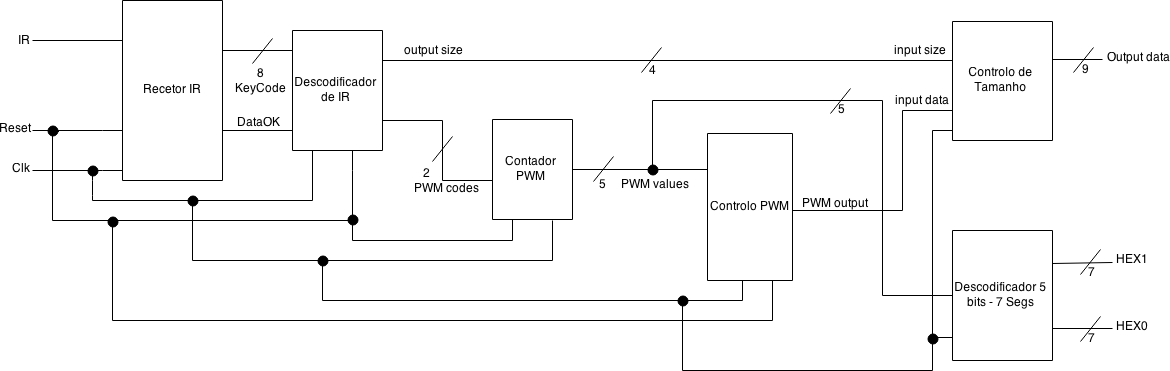
\includegraphics[height=4cm]{img/ir_leds2}}
\caption{Diagrama de blocos do projecto a desenvolver}
\label{fig:ir_leds2}
\end{figure}

\subsection{Notas Importantes}

\begin{itemize}
\item Os códigos infra-vermelhos são recebidos bit a bit pelo bloco \verb|Recetor| \verb|IR|. É responsabilidade deste assegurar a construção de um vector de 8 bits (tamanho do código correspondente a uma tecla do comando), dando indicação de quando o valor de saída é válido. Este bloco acenta numa máquina de estados conforme exemplificado na Figura \ref{fig:ir_leds2} e princípios disponiveis em \url{http://goo.gl/VjNYSf}, p.77.
\item Pulse Width Modulation (PWM) é uma técnica utilizada para obter resultados analógicos através de meios digitais. Essencialmente é criada uma onda quadrada, comutando entre ON/OFF. Variando o intervalo de tempo que o sinal está ON face ao que está a OFF, é possível simular uma variação de voltagem, permitindo a alteração de intensidade luminosa de LEDs. Um breve resumo sobre o assunto está disponível em \url{http://www.arduino.cc/en/Tutorial/PWM}.
\item Esta arquitetura é a que nos comprometemos a realizar, no entanto, caso no desenvolvimento do projeto achemos que seria interessante implementar algo mais ou de alguma forma diferente, comunicá-lo-emos ao professor responsável e em resposta afirmativa modificaremos a arquitetura de forma a incluir essas alterações. Assim, o resultado final poderá variar ligeiramente do expresso aqui, no entanto a base do trabalho deverá manter-se constante ao longo de todo o projecto.
\item Apesar de ter sido disponibilizado um descodificador de infra-vermelhos pelos docentes da unidade curricular de Laboratórios de Sistemas Digitais, pretendemos desenvolver o nosso próprio descodificador e utilizá-lo no âmbito do projeto.
\end{itemize}

\begin{figure}[ht]
\center
\fbox{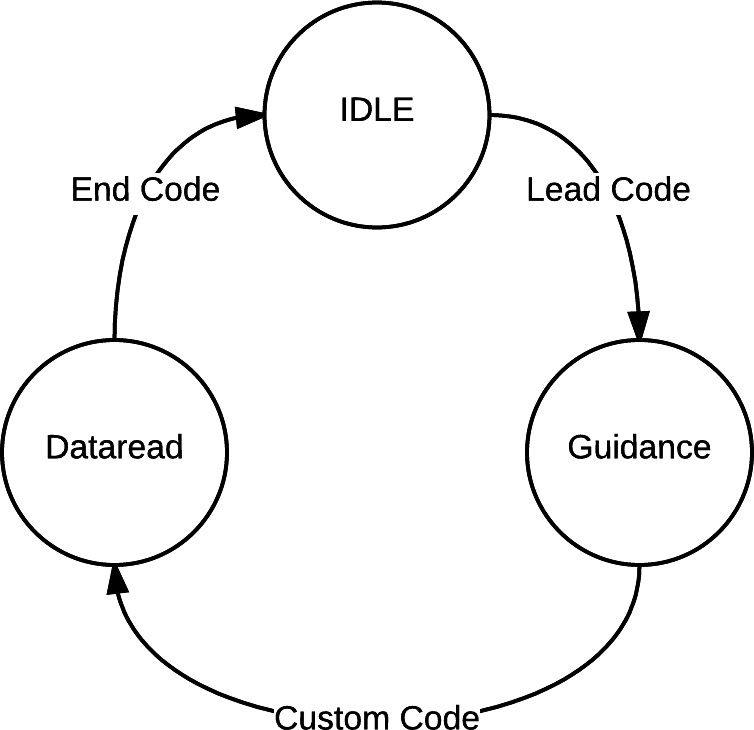
\includegraphics[height=6cm]{img/ir_leds3}}
\caption{Diagrama de estados de Recetor de IR}
\label{fig:ir_leds3}
\end{figure}

\section{Abordagem ao Desenvolvimento}

Cada bloco deverá ser desenvolvido individualmente, podendo recorrer-se a sub-blocos simples caso se veja algum interessa nesta abordagem. Todos os blocos expressos neste guião deverão ser validados. Numa primeira abordagem serão desenvolvidos os blocos \verb|Recetor IR| e \verb|Descodificador IR|. Dada a natureza estrutural destes blocos na máquina, devem passar por validações rigorosas de forma a assegurar que todo o seu funcionamente não está comprometido de raíz. Após serem obtidos resultados satisfatórios, deverão ser desenvolvidos os módulos \verb|Contador| \verb|PWM| e \verb|Controlo| \verb|PWM|, e finalmente os \verb|Descodificador| \verb|5 bits - 7 Seg| e \verb|Controlo| \verb|de Tamanho|.

Em relação aos primeiros dois blocos a serem desenvolvidos, deve-se assegurar que o sinal de infra-vermelho é corretamente recebido (o código de saída do \verb|Recetor IR| deverá corresponder aos indicados no manual de utilizador da Terasic), enquanto que as saídas do \verb|Descodificador IR| são as correctas face aos códigos introduzidos. Deverá também ser prestada especial atenção para que os blocos \verb|Contador| \verb|PWM| e \verb|Descodificador IR| comuniquem correctamente, isto é, deve assegurar-se que o contador não soma ou subtrai valores em excesso quando uma tecla é premida.

Assim, em cada fase do trabalho cada elemento do grupo deverá trabalhar num dos blocos, assegurando que o bloco desenvolvido vai de encontro ao expresso neste relatório.

\section{Manual de Utilizador}
\label{sec:Manual}

O número de LEDs acesos pode variar entre 0 e 9, sendo cada valor definido, de forma discreta, pela tecla pressionada. Já a intensidade luminosa varia de 0 a 31, sendo o seu valor definido em função do valor presente. A seta da esquerda decrementa o valor (desde que superior a 0), enquanto que a seta direita o incrementa (desde que inferior a 31). O botão POWER permite colocar a máquina em ``suspensão'', isto é, deverá colocar todos os LEDs com luminosidade 0, guardando o valor de intensidade anteriormente registado. A partir desse instante qualquer alteração na luminosidade não deverá surtir qualquer efeito. Quando o botão de POWER é premido novamente, então a intensidade guardada deverá ser devolvida aos LEDs, retomando assim o funcionamento normal da máquino. Deverá ainda existir um botão de RESET que colocará o número de LEDs acesos bem como a sua intensidade a 0. O valor da intensidade luminosa deverá também ser exposto em dois displays de sete segmentos, em base decimal.

\begin{itemize}
\item A Figura \ref{fig:ir_leds0} demonstra os controlos do comando admitidos, bem como as suas funções.
\item Os LEDs controlados são os 9 verdes (numerados de 0 a 8).
\item Em qualquer instante a intensidade luminosa dos LEDs será mostrada nos displays de sete segmentos HEX1 e HEX0.
\item Clicar no botão KEY0 do kit fará o reset da máquina.
\end{itemize}

\begin{figure}[ht]
\center
\fbox{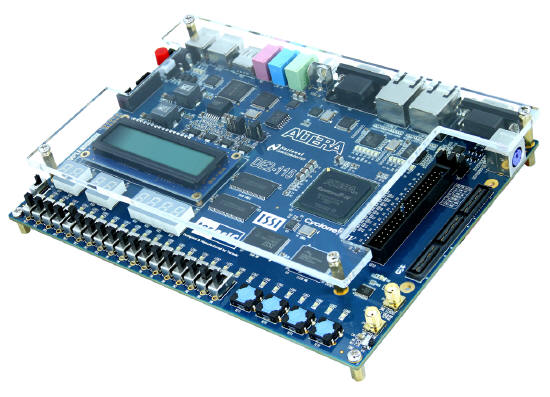
\includegraphics[height=7cm]{img/ir_leds0}}
\caption{Funções suportadas do comando utilizado}
\label{fig:ir_leds0}
\end{figure}

\maketitle
\nocite{*}

\end{document}
